%%%%%%%%%%%%%%%%%%%%%%%%%%%%%%%%%%%%%%%%%%%%%%%%%%%%%%%%%%%%%%%
%% OXFORD THESIS TEMPLATE

% Use this template to produce a standard thesis that meets the Oxford University requirements for DPhil submission
%
% Originally by Keith A. Gillow (gillow@maths.ox.ac.uk), 1997
% Modified by Sam Evans (sam@samuelevansresearch.org), 2007
% Modified by John McManigle (john@oxfordechoes.com), 2015
% Modified by Ulrik Lyngs (ulrik.lyngs@cs.ox.ac.uk), 2018-, for use with R Markdown
%
% Ulrik Lyngs, 25 Nov 2018: Following John McManigle, broad permissions are granted to use, modify, and distribute this software
% as specified in the MIT License included in this distribution's LICENSE file.
%
% John commented this file extensively, so read through to see how to use the various options.  Remember that in LaTeX,
% any line starting with a % is NOT executed.  Several places below, you have a choice of which line to use
% out of multiple options (eg draft vs final, for PDF vs for binding, etc.)  When you pick one, add a % to the beginning of
% the lines you don't want.


%%%%% PAGE LAYOUT
% The most common choices should be below.  You can also do other things, like replacing "a4paper" with "letterpaper", etc.

% This one formats for two-sided binding (ie left and right pages have mirror margins; blank pages inserted where needed):
%\documentclass[a4paper,twoside]{templates/ociamthesis}
% This one formats for one-sided binding (ie left margin > right margin; no extra blank pages):
%\documentclass[a4paper]{ociamthesis}
% This one formats for PDF output (ie equal margins, no extra blank pages):
%\documentclass[a4paper,nobind]{templates/ociamthesis}

% As you can see from the uncommented line below, oxforddown template uses the a4paper size, 
% and passes in the binding option from the YAML header in index.Rmd:
\documentclass[a4paper, nobind]{templates/ociamthesis}


%%%%% ADDING LATEX PACKAGES
% add hyperref package with options from YAML %
\usepackage[pdfpagelabels]{hyperref}
% change the default coloring of links to something sensible
\usepackage{xcolor}

\definecolor{myurlcolor}{RGB}{0,0,139}
\definecolor{mycitecolor}{RGB}{0,33,71}

\hypersetup{
  hidelinks,
  colorlinks,
  linkcolor=.,
  urlcolor=myurlcolor,
  citecolor=mycitecolor
}



% add float package to allow manual control of figure positioning %
\usepackage{float}

% enable strikethrough
\usepackage[normalem]{ulem}

% use soul package for correction highlighting
\usepackage{color, soul}
\definecolor{correctioncolor}{HTML}{CCCCFF}
\sethlcolor{correctioncolor}
\newcommand{\ctext}[3][RGB]{%
  \begingroup
  \definecolor{hlcolor}{#1}{#2}\sethlcolor{hlcolor}%
  \hl{#3}%
  \endgroup
}
\soulregister\ref7
\soulregister\cite7
\soulregister\autocite7
\soulregister\textcite7
\soulregister\pageref7

%%%%% FIXING / ADDING THINGS THAT'S SPECIAL TO R MARKDOWN'S USE OF LATEX TEMPLATES
% pandoc puts lists in 'tightlist' command when no space between bullet points in Rmd file,
% so we add this command to the template
\providecommand{\tightlist}{%
  \setlength{\itemsep}{0pt}\setlength{\parskip}{0pt}}
 
% UL 1 Dec 2018, fix to include code in shaded environments

% User-included things with header_includes or in_header will appear here
% kableExtra packages will appear here if you use library(kableExtra)
\usepackage{booktabs}
\usepackage{longtable}
\usepackage{array}
\usepackage{multirow}
\usepackage{wrapfig}
\usepackage{float}
\usepackage{colortbl}
\usepackage{pdflscape}
\usepackage{tabu}
\usepackage{threeparttable}
\usepackage{threeparttablex}
\usepackage[normalem]{ulem}
\usepackage{makecell}
\usepackage{xcolor}


%UL set section header spacing
\usepackage{titlesec}
% 
\titlespacing\subsubsection{0pt}{24pt plus 4pt minus 2pt}{0pt plus 2pt minus 2pt}


%UL set whitespace around verbatim environments
\usepackage{etoolbox}
\makeatletter
\preto{\@verbatim}{\topsep=0pt \partopsep=0pt }
\makeatother



%%%%%%% PAGE HEADERS AND FOOTERS %%%%%%%%%
\usepackage{fancyhdr}
\setlength{\headheight}{15pt}
\fancyhf{} % clear the header and footers
\pagestyle{fancy}
\renewcommand{\chaptermark}[1]{\markboth{\thechapter. #1}{\thechapter. #1}}
\renewcommand{\sectionmark}[1]{\markright{\thesection. #1}} 
\renewcommand{\headrulewidth}{0pt}

\fancyhead[LO]{\emph{\leftmark}} 
\fancyhead[RE]{\emph{\rightmark}} 

% UL page number position 
\fancyfoot[C]{\emph{\thepage}} %regular pages
\fancypagestyle{plain}{\fancyhf{}\fancyfoot[C]{\emph{\thepage}}} %chapter pages

% JEM fix header on cleared pages for openright
\def\cleardoublepage{\clearpage\if@twoside \ifodd\c@page\else
   \hbox{}
   \fancyfoot[C]{}
   \newpage
   \if@twocolumn\hbox{}\newpage
   \fi
   \fancyhead[LO]{\emph{\leftmark}} 
   \fancyhead[RE]{\emph{\rightmark}} 
   \fi\fi}


%%%%% SELECT YOUR DRAFT OPTIONS
% This adds a "DRAFT" footer to every normal page.  (The first page of each chapter is not a "normal" page.)

% IP feb 2021: option to include line numbers in PDF

% This highlights (in blue) corrections marked with (for words) \mccorrect{blah} or (for whole
% paragraphs) \begin{mccorrection} . . . \end{mccorrection}.  This can be useful for sending a PDF of
% your corrected thesis to your examiners for review.  Turn it off, and the blue disappears.
\correctionstrue


%%%%% BIBLIOGRAPHY SETUP
% Note that your bibliography will require some tweaking depending on your department, preferred format, etc.
% If you've not used LaTeX before, I recommend reading a little about biblatex/biber and getting started with it.
% If you're already a LaTeX pro and are used to natbib or something, modify as necessary.
% Either way, you'll have to choose and configure an appropriate bibliography format...


\usepackage[style=authoryear, sorting=nyt, backend=biber, maxcitenames=2, useprefix, doi=true, isbn=false, uniquename=false]{biblatex}
\newcommand*{\bibtitle}{Works Cited}

\addbibresource{bibliography/references.bib}
\addbibresource{bibliography/additional-references.bib}


% This makes the bibliography left-aligned (not 'justified') and slightly smaller font.
\renewcommand*{\bibfont}{\raggedright\small}


% Uncomment this if you want equation numbers per section (2.3.12), instead of per chapter (2.18):
%\numberwithin{equation}{subsection}


%%%%% THESIS / TITLE PAGE INFORMATION
% Everybody needs to complete the following:
\title{Bacterial filamentation: a bet for survival in stressful environments}
\author{Jesús Vélez Santiago}
\college{Center for Genomic Sciences}

% Master's candidates who require the alternate title page (with candidate number and word count)
% must also un-comment and complete the following three lines:

% Uncomment the following line if your degree also includes exams (eg most masters):
%\renewcommand{\submittedtext}{Submitted in partial completion of the}
% Your full degree name.  (But remember that DPhils aren't "in" anything.  They're just DPhils.)
\degree{Bachelor of Science}
% Term and year of submission, or date if your board requires (eg most masters)
\degreedate{Cuernavaca, Morelos, Mexico - 2021-08}


%%%%% YOUR OWN PERSONAL MACROS
% This is a good place to dump your own LaTeX macros as they come up.

% To make text superscripts shortcuts
	\renewcommand{\th}{\textsuperscript{th}} % ex: I won 4\th place
	\newcommand{\nd}{\textsuperscript{nd}}
	\renewcommand{\st}{\textsuperscript{st}}
	\newcommand{\rd}{\textsuperscript{rd}}

%%%%% THE ACTUAL DOCUMENT STARTS HERE
\begin{document}

%%%%% CHOOSE YOUR LINE SPACING HERE
% This is the official option.  Use it for your submission copy and library copy:
\setlength{\textbaselineskip}{22pt plus2pt}
% This is closer spacing (about 1.5-spaced) that you might prefer for your personal copies:
%\setlength{\textbaselineskip}{18pt plus2pt minus1pt}

% You can set the spacing here for the roman-numbered pages (acknowledgements, table of contents, etc.)
\setlength{\frontmatterbaselineskip}{17pt plus1pt minus1pt}

% UL: You can set the line and paragraph spacing here for the separate abstract page to be handed in to Examination schools
\setlength{\abstractseparatelineskip}{13pt plus1pt minus1pt}
\setlength{\abstractseparateparskip}{0pt plus 1pt}

% UL: You can set the general paragraph spacing here - I've set it to 2pt (was 0) so
% it's less claustrophobic
\setlength{\parskip}{2pt plus 1pt}

%
% Oxford University logo on title page
%
\def\crest{{
\includegraphics[width=5cm]{figures/logos/unam.pdf}}}
\renewcommand{\university}{National Autonomous University of Mexico}
\renewcommand{\submittedtext}{A thesis submitted for the degree of}


% Leave this line alone; it gets things started for the real document.
\setlength{\baselineskip}{\textbaselineskip}


%%%%% CHOOSE YOUR SECTION NUMBERING DEPTH HERE
% You have two choices.  First, how far down are sections numbered?  (Below that, they're named but
% don't get numbers.)  Second, what level of section appears in the table of contents?  These don't have
% to match: you can have numbered sections that don't show up in the ToC, or unnumbered sections that
% do.  Throughout, 0 = chapter; 1 = section; 2 = subsection; 3 = subsubsection, 4 = paragraph...

% The level that gets a number:
\setcounter{secnumdepth}{2}
% The level that shows up in the ToC:
\setcounter{tocdepth}{1}


%%%%% ABSTRACT SEPARATE
% This is used to create the separate, one-page abstract that you are required to hand into the Exam
% Schools.  You can comment it out to generate a PDF for printing or whatnot.

% JEM: Pages are roman numbered from here, though page numbers are invisible until ToC.  This is in
% keeping with most typesetting conventions.
\begin{romanpages}

% Title page is created here
\maketitle

%%%%% DEDICATION -- If you'd like one, un-comment the following.
\begin{dedication}
  For Yihui Xie
\end{dedication}

%%%%% ACKNOWLEDGEMENTS -- Nothing to do here except comment out if you don't want it.
\begin{acknowledgements}
 	Lorem ipsum dolor sit amet, consectetur adipiscing elit. Integer tristique, sem egestas aliquam varius, arcu nisi ullamcorper lacus, quis convallis enim velit et arcu. Vestibulum lacus arcu, tempor non dapibus vitae, malesuada ut ipsum. Phasellus condimentum diam ex. Sed maximus a mauris vel aliquet.

  Integer neque sapien, cursus eu viverra consequat, cursus congue dui. Maecenas est dui, rutrum vitae enim vel, varius scelerisque tortor. In vel dignissim orci. Integer varius neque mauris, mollis commodo libero fringilla sed. Nunc accumsan, libero id interdum dignissim, nulla nibh consectetur lorem, vel dignissim erat magna vitae ante. Aliquam at est lectus. Suspendisse nec sem euismod, condimentum neque sit amet, malesuada nibh. Aenean condimentum pharetra quam, id venenatis mauris tempor a.

  \begin{flushright}
  Jesús Vélez Santiago \\
  Center for Genomic Sciences \\
  2021, 08
  \end{flushright}
\end{acknowledgements}


%%%%% ABSTRACT -- Nothing to do here except comment out if you don't want it.
\begin{abstract}
	Etiam venenatis purus eu felis viverra sodales. Sed et varius ex. Nullam sit amet aliquet purus. Fusce elementum vitae est eget vulputate. Aliquam erat volutpat. Donec ac suscipit leo, sed euismod nisi. Duis malesuada elementum pulvinar. Ut et vulputate augue. In dignissim ligula at nulla feugiat cursus. Suspendisse sed diam ut ligula sollicitudin pellentesque. Etiam ut gravida velit, vitae lobortis mi. Nam congue laoreet mauris sit amet iaculis.
\end{abstract}

%%%%% MINI TABLES
% This lays the groundwork for per-chapter, mini tables of contents.  Comment the following line
% (and remove \minitoc from the chapter files) if you don't want this.  Un-comment either of the
% next two lines if you want a per-chapter list of figures or tables.
  \dominitoc % include a mini table of contents

% This aligns the bottom of the text of each page.  It generally makes things look better.
\flushbottom

% This is where the whole-document ToC appears:
\tableofcontents

\listoffigures
	\mtcaddchapter
  	% \mtcaddchapter is needed when adding a non-chapter (but chapter-like) entity to avoid confusing minitoc

% Uncomment to generate a list of tables:
\listoftables
  \mtcaddchapter
%%%%% LIST OF ABBREVIATIONS
% This example includes a list of abbreviations.  Look at text/abbreviations.tex to see how that file is
% formatted.  The template can handle any kind of list though, so this might be a good place for a
% glossary, etc.
% First parameter can be changed eg to "Glossary" or something.
% Second parameter is the max length of bold terms.
\begin{mclistof}{List of Abbreviations}{3.2cm}

\item[1-D, 2-D]

One- or two-dimensional, referring \textbf{in this thesis} to spatial dimensions in an image.

\item[Otter]

One of the finest of water mammals.

\item[Hedgehog]

Quite a nice prickly friend.

\end{mclistof} 


% The Roman pages, like the Roman Empire, must come to its inevitable close.
\end{romanpages}

%%%%% CHAPTERS
% Add or remove any chapters you'd like here, by file name (excluding '.tex'):
\flushbottom

% all your chapters and appendices will appear here
\hypertarget{introduction}{%
\chapter*{Introduction}\label{introduction}}
\addcontentsline{toc}{chapter}{Introduction}

\adjustmtc
\markboth{Introduction}{}

\hypertarget{experiment-analysis}{%
\chapter{Experiment analysis}\label{experiment-analysis}}

\minitoc 

\hypertarget{introduction-1}{%
\section{Introduction}\label{introduction-1}}

\hypertarget{experiment-design}{%
\section{Experiment design}\label{experiment-design}}

\hypertarget{exploratory-data-analysis}{%
\section{Exploratory Data Analysis}\label{exploratory-data-analysis}}

\hypertarget{cells-level}{%
\subsection{Cells level}\label{cells-level}}



\begin{figure}[H]
\includegraphics[width=1\linewidth]{downloadFigs4latex__main/03-cells-distribution-across-experiments} \caption{\textbf{Cell distribution across experiments.}}\label{fig:03-cells-distribution-across-experiments}
\end{figure}



\begin{figure}[H]
\includegraphics[width=1\linewidth]{downloadFigs4latex__main/03-cells-life-time-classes-distribution-1} \caption{\textbf{Cells life time classes distribution.}}\label{fig:03-cells-life-time-classes-distribution-1}
\end{figure}



\begin{figure}[H]
\includegraphics[width=1\linewidth]{downloadFigs4latex__main/03-division-number-divisions-1} \caption{\textbf{Cell's number of divisions.}}\label{fig:03-division-number-divisions-1}
\end{figure}



\begin{figure}[H]
\includegraphics[width=1\linewidth]{downloadFigs4latex__main/03-division-time-since-last-division-1} \caption{\textbf{Time since last division}}\label{fig:03-division-time-since-last-division-1}
\end{figure}



\begin{figure}[H]
\includegraphics[width=1\linewidth]{downloadFigs4latex__main/03-focus-just-in-initial-values-1} \caption{\textbf{Experiment initial values}}\label{fig:03-focus-just-in-initial-values-1}
\end{figure}



\begin{figure}[H]
\includegraphics[width=1\linewidth]{downloadFigs4latex__main/03-metric-differences-1} \caption{\textbf{Experiment initial values differences.}}\label{fig:03-metric-differences-1}
\end{figure}



\begin{figure}[H]
\includegraphics[width=1\linewidth]{downloadFigs4latex__main/03-see-datasets-individualy-pca-chromosome-points-in-new-coordinates-1} \caption{\textbf{Chromosome PCA.}}\label{fig:03-see-datasets-individualy-pca-chromosome-points-in-new-coordinates-1}
\end{figure}



\begin{figure}[H]
\includegraphics[width=1\linewidth]{downloadFigs4latex__main/03-see-datasets-individualy-pca-chromosome-variable-contribution-1} \caption{\textbf{Chromosome PCA variables contribution.}}\label{fig:03-see-datasets-individualy-pca-chromosome-variable-contribution-1}
\end{figure}



\begin{figure}[H]
\includegraphics[width=1\linewidth]{downloadFigs4latex__main/03-see-datasets-individualy-pca-plasmid-points-in-new-coordinates-1} \caption{\textbf{Plasmid PCA}}\label{fig:03-see-datasets-individualy-pca-plasmid-points-in-new-coordinates-1}
\end{figure}



\begin{figure}[H]
\includegraphics[width=1\linewidth]{downloadFigs4latex__main/03-see-datasets-individualy-pca-plasmid-variable-contribution-1} \caption{\textbf{Plasmid PCA variables contribution.}}\label{fig:03-see-datasets-individualy-pca-plasmid-variable-contribution-1}
\end{figure}



\begin{figure}[H]
\includegraphics[width=1\linewidth]{downloadFigs4latex__main/03-see-datasets-individualy-umap-chromosome-points-in-new-coordinates-1} \caption{\textbf{UMAP of Chromosome experiment.}}\label{fig:03-see-datasets-individualy-umap-chromosome-points-in-new-coordinates-1}
\end{figure}



\begin{figure}[H]
\includegraphics[width=1\linewidth]{downloadFigs4latex__main/3-see-datasets-individualy-umap-plasmid-points-in-new-coordinates-1} \caption{\textbf{UMAP of Plasmid experiment.}}\label{fig:3-see-datasets-individualy-umap-plasmid-points-in-new-coordinates-1}
\end{figure}



\begin{figure}[H]
\includegraphics[width=1\linewidth]{downloadFigs4latex__main/03-temporal-metric-distribution-ds-red-1} \caption{\textbf{DS-red temporal distribution.}}\label{fig:03-temporal-metric-distribution-ds-red-1}
\end{figure}



\begin{figure}[H]
\includegraphics[width=1\linewidth]{downloadFigs4latex__main/03-temporal-metric-distribution-gfp-1} \caption{\textbf{GFP temporal distribution.}}\label{fig:03-temporal-metric-distribution-gfp-1}
\end{figure}



\begin{figure}[H]
\includegraphics[width=1\linewidth]{downloadFigs4latex__main/03-temporal-metric-distribution-length-1} \caption{\textbf{Length temporal distribution.}}\label{fig:03-temporal-metric-distribution-length-1}
\end{figure}



\begin{figure}[H]
\includegraphics[width=1\linewidth]{downloadFigs4latex__main/03-time-to-filamentation-all-1} \caption{\textbf{Time to filamentation without filters.}}\label{fig:03-time-to-filamentation-all-1}
\end{figure}



\begin{figure}[H]
\includegraphics[width=1\linewidth]{downloadFigs4latex__main/03-time-to-filamentation-filamented-once-experiment-start-1} \caption{\textbf{Time to filamentation filtered.}}\label{fig:03-time-to-filamentation-filamented-once-experiment-start-1}
\end{figure}



\begin{figure}[H]
\includegraphics[width=1\linewidth]{downloadFigs4latex__main/03-time-to-filamentation-include-time-to-filamentation-in-initial-exploration-diff-values-1} \caption{\textbf{Experiment initial values differences with time.}}\label{fig:03-time-to-filamentation-include-time-to-filamentation-in-initial-exploration-diff-values-1}
\end{figure}



\begin{figure}[H]
\includegraphics[width=1\linewidth]{downloadFigs4latex__main/03-time-to-filamentation-include-time-to-filamentation-in-initial-exploration-initial-values-1} \caption{\textbf{Experiment initial values with time.}}\label{fig:03-time-to-filamentation-include-time-to-filamentation-in-initial-exploration-initial-values-1}
\end{figure}

\hypertarget{tracks-level}{%
\subsection{Tracks level}\label{tracks-level}}



\begin{figure}[H]
\includegraphics[width=1\linewidth]{downloadFigs4latex__main/04-metrics-over-time-1} \caption{\textbf{Population measurements over time.}}\label{fig:04-metrics-over-time-1}
\end{figure}



\begin{figure}[H]
\includegraphics[width=1\linewidth]{downloadFigs4latex__main/04-length-survival-probability-1} \caption{\textbf{Plasmid initial GFP survival probability.}}\label{fig:04-length-survival-probability-1}
\end{figure}



\begin{figure}[H]
\includegraphics[width=1\linewidth]{downloadFigs4latex__main/04-gfp-survival-probability-1} \caption{\textbf{Plasmid initial length survival probability.}}\label{fig:04-gfp-survival-probability-1}
\end{figure}



\begin{figure}[H]
\includegraphics[width=1\linewidth]{downloadFigs4latex__main/04-cell-status-over-time-status-without-dead-1} \caption{\textbf{Population status over time without dead.}}\label{fig:04-cell-status-over-time-status-without-dead-1}
\end{figure}



\begin{figure}[H]
\includegraphics[width=1\linewidth]{downloadFigs4latex__main/04-cell-status-over-time-status-with-dead-1} \caption{\textbf{Population status over time with dead.}}\label{fig:04-cell-status-over-time-status-with-dead-1}
\end{figure}



\begin{figure}[H]
\includegraphics[width=1\linewidth]{downloadFigs4latex__main/04-cell-status-over-time-proportion-living-cells-by-gfp-row-1} \caption{\textbf{Population survivals binned by initial GFP over time.}}\label{fig:04-cell-status-over-time-proportion-living-cells-by-gfp-row-1}
\end{figure}



\begin{figure}[H]
\includegraphics[width=1\linewidth]{downloadFigs4latex__main/04-cell-status-over-time-proportion-living-cells-by-gfp-point-1} \caption{\textbf{Normalized population survivals binned by initial GFP over time.}}\label{fig:04-cell-status-over-time-proportion-living-cells-by-gfp-point-1}
\end{figure}

\hypertarget{discussion}{%
\section{Discussion}\label{discussion}}

\hypertarget{filamentation-abstraction}{%
\chapter{Models to the rescue; filamentation abstraction}\label{filamentation-abstraction}}

\minitoc 

\noindent Scientists have extensively studied the mechanisms that orchestrate the growth and division of bacterial cells. Cells adapt their shape and dimensions in response to variations in the intracellular and extracellular environments by integrating information about the presence of nutrients or harmful agents in the decision to grow or divide. Filamentation is a process that occurs when rod-shaped cells stop dividing but continue to grow, thus producing elongated cells. Some cells can naturally grow as filamentous, while others only do so under stressful conditions. Here we use mathematical modeling and computational simulations to evaluate a toxic agent's intracellular concentration as a function of cell length. We show that filamentation can act as a strategy that promotes the resilience of a bacterial population under stressful environmental conditions.

\hypertarget{introduction-2}{%
\section{Introduction}\label{introduction-2}}

By integrating information from the environment, cells can alter their cell cycle. For instance, some cells arrest the cell division in the presence of toxic agents but continue to grow. Previous studies have shown that this filamentation phenomenon provides a mechanism that enables cells to cope with stress, which leads to an increase in the probability of survival \autocite{justiceMorphologicalPlasticityBacterial2008}. For example, filamentation can be a process capable of subverting innate defenses during urinary tract infection, facilitating the transition of additional rounds of intracellular bacterial community formation \autocite{justiceFilamentationEscherichiaColi2006}.

Although filament growth can help mitigate environmental stress (e.g., by activating the SOS response system \autocite{justiceMorphologicalPlasticityBacterial2008}), the evolutionary benefits of producing elongated cells that do not divide are unclear. Here, we proposed a mathematical model based on ordinary differential equations that explicitly considers the concentration of intracellular toxin as a function of the cell's length (see Equation \eqref{eq:model-equation}). The model is built based on the growth ratio of measurements of the surface area (\(SA\)) and the cell volume (\(V\)), whereby the uptake rate of the toxin depends on the \(SA\). However, \(V's\) rate of change for \(SA\) is higher than \(SA\) for \(V\), which results in a transient reduction in the intracellular toxin concentration (see Figure \ref{fig:cell-dimensions-relationship}). Therefore, we hypothesized that this geometric interpretation of filamentation represents a biophysical defense line to increase the probability of a bacterial population's survival in response to stressful environments.





\begin{figure}[H]
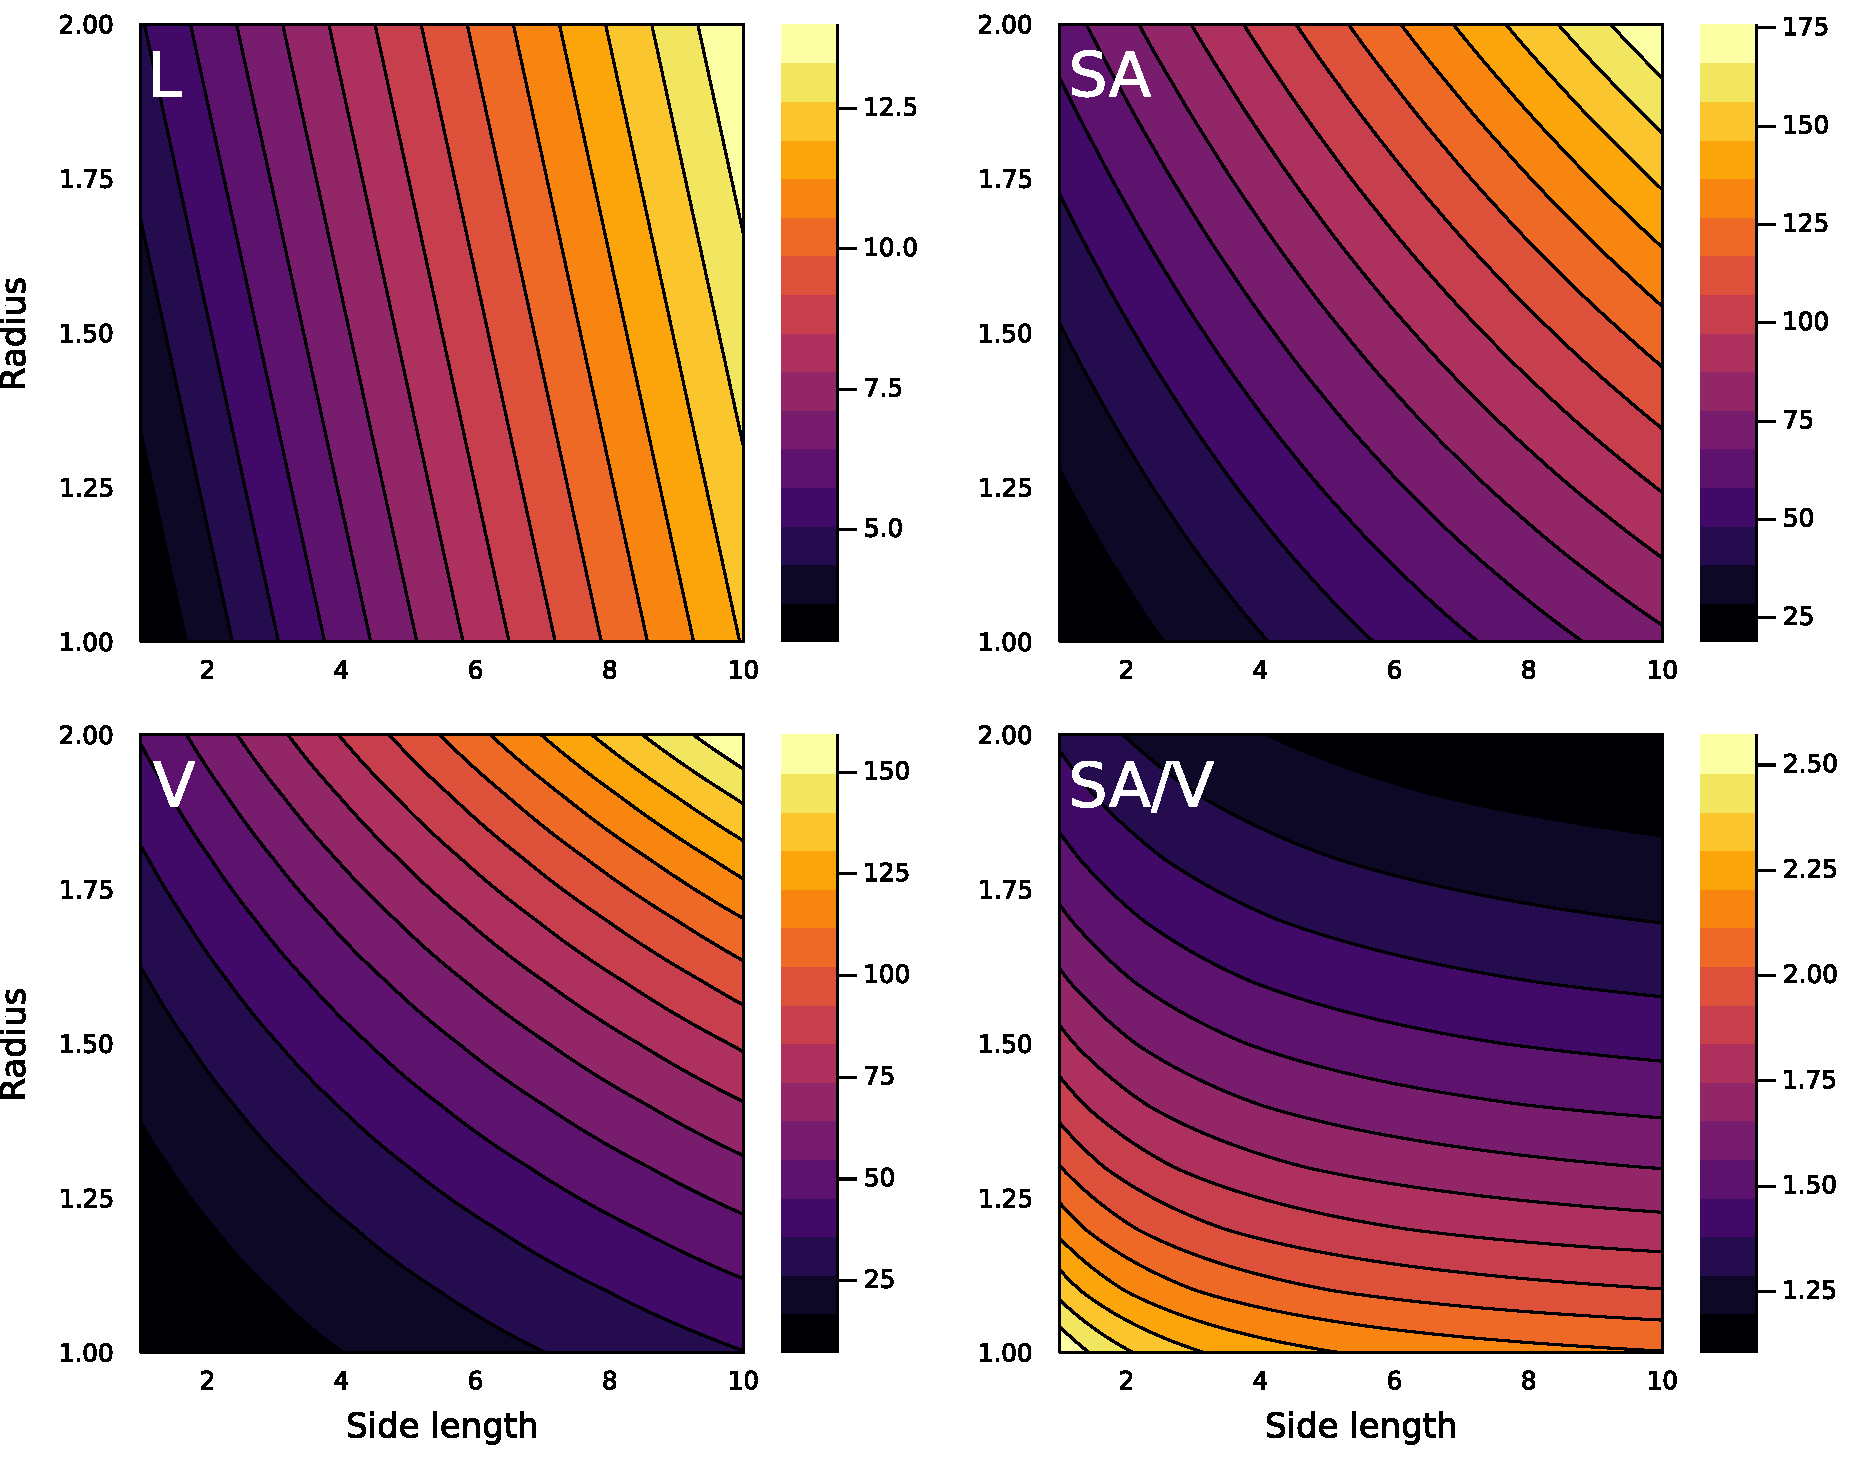
\includegraphics[width=1\linewidth]{downloadFigs4latex__main/cell-dimensions-relationship} \caption[Cell dimensions relationship.]{\textbf{Cell dimensions relationship.}}\label{fig:cell-dimensions-relationship}
\end{figure}

\hypertarget{filamentation-model}{%
\section{Filamentation model}\label{filamentation-model}}

Let us assume the shape of cells is a cylinder with hemispherical ends. Based on this geometric structure, a nonlinear system of differential equations governing filamentation can be written as follows:

\begin{equation}
\begin{split}
\frac{dT_{int}}{dt} &= T_{sa} \cdot (T_{ext}(t) - T_{vol}) - \alpha \cdot T_{ant} \cdot T_{int} \\
\frac{dL}{dt} &= 
  \begin{cases} 
    \beta \cdot L,& \text{if } T_{int} \geq T_{sos},  t \geq \tau_{sos} + \tau_{delay} \text{ and } L < L_{max}  \\
    0,            & \text{otherwise}
  \end{cases}
\end{split}
\label{eq:model-equation}
\end{equation}

It considers the internal toxin (\(T_{int}\)) and the cell length (\(L\)) as variables. \(T_{sa}\) and \(T_{vol}\) represent the surface area and volume of the toxin in the cell, respectively. \(T_{ext}(t)\) is a function that returns the amount of toxin in the cell medium. \(T_{anti}\) and \(\alpha\) symbolize the amount of antitoxin and its efficiency rate, respectively. \(\beta\) as the rate of filamentation. \(L_{max}\) is the maximum size that the cell can reach when filamentation is on. \(T_{sos}\) and \(T_{kill}\) are thresholds for filamentation and death, respectively. Finally, \(\tau_{delay}\) is the amount of time required to activate filamentation after reaching the \(T_{sos}\) threshold.

\hypertarget{results}{%
\section{Results}\label{results}}

\hypertarget{filamentation-provides-transient-resistance-under-stressful-conditions}{%
\subsection{Filamentation provides transient resistance under stressful conditions}\label{filamentation-provides-transient-resistance-under-stressful-conditions}}

When growing rod-shaped bacterial cells under constant conditions, the distribution of lengths and radii is narrow \autocite{schaechterGrowthCellNuclear1962}. However, when growing under stress conditions, some cells produce filaments \autocite{schaechterDependencyMediumTemperature1958}. This phenomenon may depend on the SOS response system \autocite{bosEmergenceAntibioticResistance2015}, which can repair DNA damage, giving the cell greater chances of recovering and surviving under stress conditions. Besides, the SOS response has been reported to have precise temporal coordination in individual bacteria \autocite{friedmanPreciseTemporalModulation2005}. Among the stress conditions that can trigger the SOS response is exposure to beta-lactam antibiotics \autocite{millerSOSResponseInduction2004}.

In general, filamentation has been studied as an unavoidable consequence of stress. However, we considered filamentation an active process that produces the first line of defense against toxic agents. Therefore, a differential equation model was proposed that assesses the change in the amount of internal toxin as a function of cell length. At the core of this model, we include the intrinsic relationship between the surface area and the capsule volume since it is vital in determining cell size \autocite{harrisRelativeRatesSurface2016}.

In figure \ref{fig:filamentation-model-ramp-signal}, cells grow in a ramp-shaped external toxin signal without considering a toxin-antitoxin system. As time progresses, the toxin in the external environment increases, so the cell raises its internal toxin levels. At approximately time \(22\), any cell reaches \(T_{sos}\). The control cell (unable to filament) and the average cell (capable of filamenting) reach the death threshold, \(T_{kill}\), at times \(31\) and \(93\) (hatched and solid black lines), respectively. Therefore, under this example, the cell has increased its life span three times more than in control by growing as a filament (green shaded area versus orange shaded area). In turn, figure \ref{fig:filamentation-model-ramp-signal} also shows stochastic simulations of the system in the intake of internal toxins. Considering that cell growth and death processes are inherently stochastic, stochastic simulations would be a better approximation. However, from now on, we will continue with the study of the deterministic model.





\begin{figure}[H]
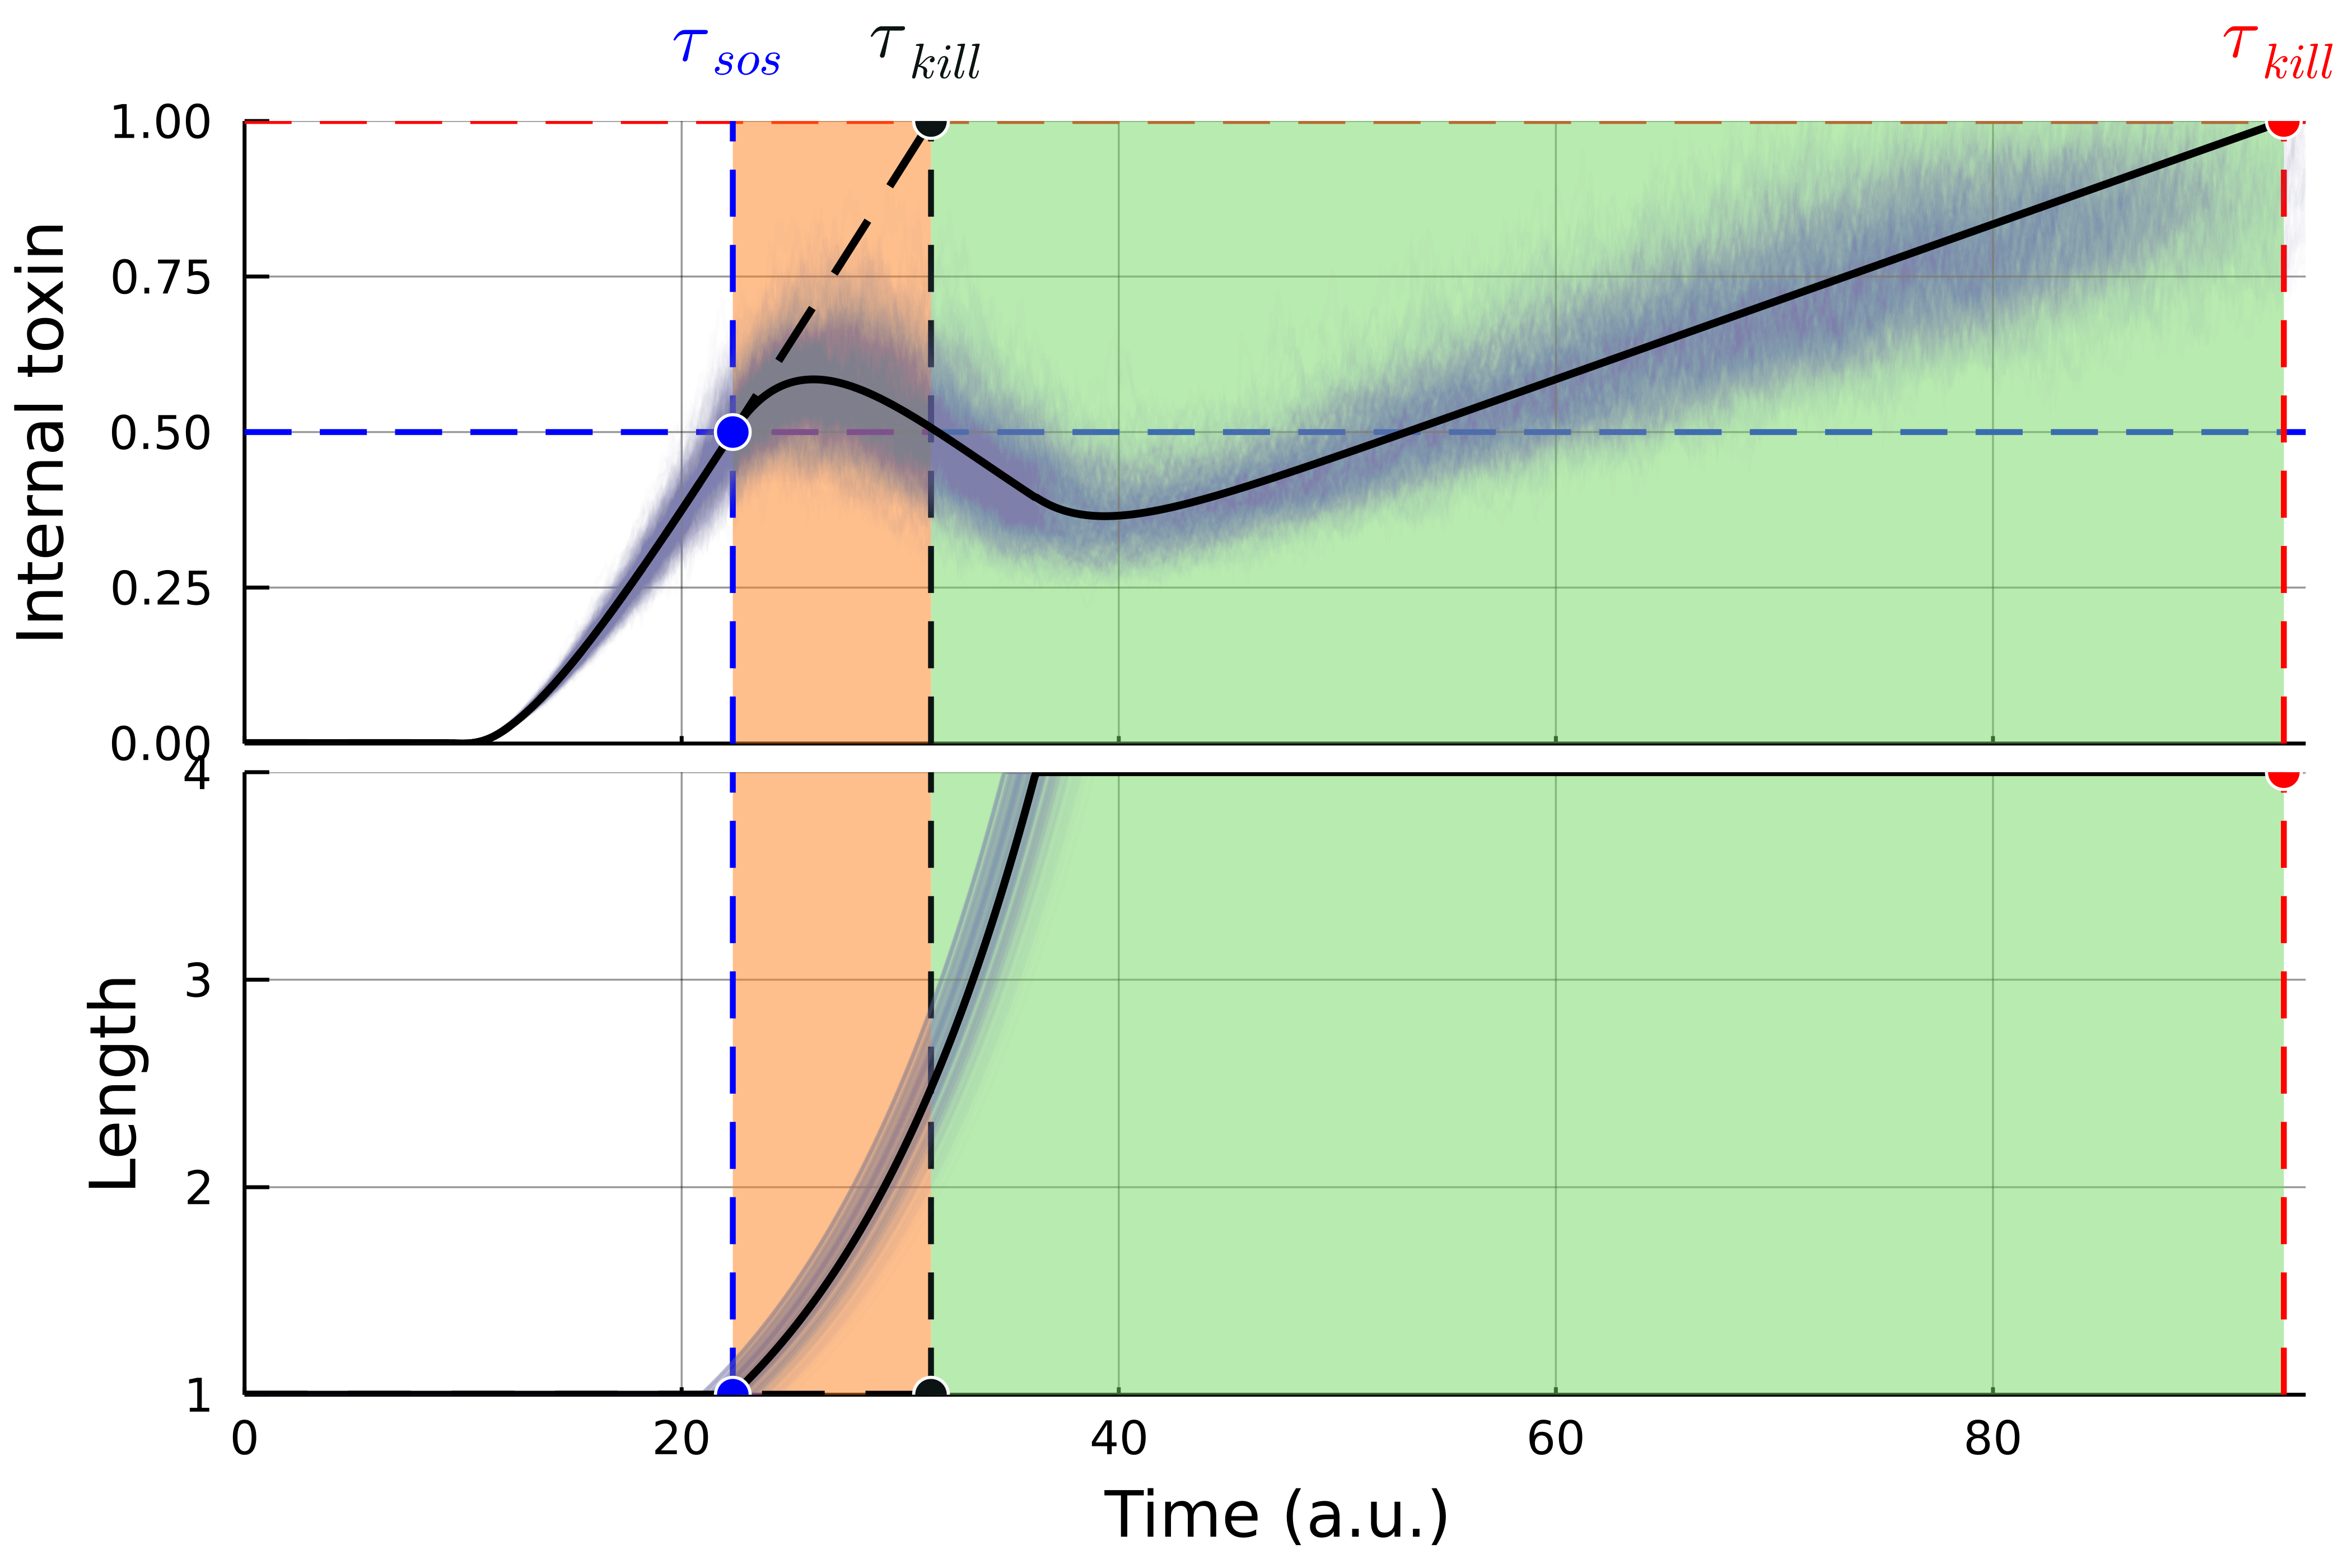
\includegraphics[width=1\linewidth]{downloadFigs4latex__main/filamentation-model-ramp-signal} \caption[Effect of filamentation on intracellular toxin concentration.]{\textbf{Effect of filamentation on intracellular toxin concentration.} In the presence of an extracellular toxic agent, the intracellular concentration of the toxin (\(T_{int}\)) increases until reaching a damage threshold that triggers filamentation (\(T_{sos}\), blue point), increasing cell length (\(L\)). When filamentation is on, the cell decreases \(T_{int}\) due to the intrinsic relationship between surface area and cell volume. When the cell reaches its maximum length, it eventually dies if the stressful stimulus is not removed (\(T_{kill}\), red dot). The hatched line represents a cell that can not grow as filament. The orange shaded area is the time between stress and the non-filament cell's death, while the green shaded area represents the temporal gain for doing so. The blue background lines represent stochastic simulations of the same system.}\label{fig:filamentation-model-ramp-signal}
\end{figure}

\hypertarget{filamentation-increases-the-minimum-inhibitory-concentration}{%
\subsection{Filamentation increases the minimum inhibitory concentration}\label{filamentation-increases-the-minimum-inhibitory-concentration}}

Antimicrobial resistance (AMR) can be considered one of the most critical health problems of the century. That is, microorganisms' ability to grow despite exposure to substances designed to inhibit their growth or kill them. In April 2014, the World Health Organization (WHO) published its first global report on AMR surveillance \autocite{EditorialBoard2014}. Taking out of the darkness a common fear, a possible post-antibiotic future in which common infections or minor injuries can kill. Therefore, understanding the mechanisms of avoiding antibiotic action is essential for producing knowledge and developing strategies that reduce the generation of resistant bacteria.

A classic experiment in laboratories finds the concentration that inhibits bacterial growth through exposure to different toxin doses. The concentration found is known as the minimum inhibitory concentration (MIC) \autocite{andrewsDeterminationMinimumInhibitory2002}. Bacteria are capable of modifying their MIC through various mechanisms, for example, mutations \autocite{lambertBacterialResistanceAntibiotics2005}, impaired membrane permeability \autocite{satoOuterMembranePermeability1991}, flux pumps \autocite{webberImportanceEffluxPumps2003}, toxin-inactivating enzymes \autocite{wrightBacterialResistanceAntibiotics2005}, and plasticity phenotypic \autocite{justiceMorphologicalPlasticityBacterial2008}. The latter is our phenomenon of interest because it considers the change in shape and size, allowing us to study it as a strategy to promote bacterial survival.

We decided to analyze the MIC change caused by filamentation through stable exposure experiments of different toxin amounts at other exposure times. Computational simulations show that when comparing cells unable to filament with those that can, there is an increase in the capacity to tolerate more generous amounts of toxin, increasing their MIC (see Figure \ref{fig:increased-time-resistance}). Therefore, it confers a gradual increase in resistance beyond filamentation's role in improving the cell's life span as the exposure time is longer.





\begin{figure}[H]
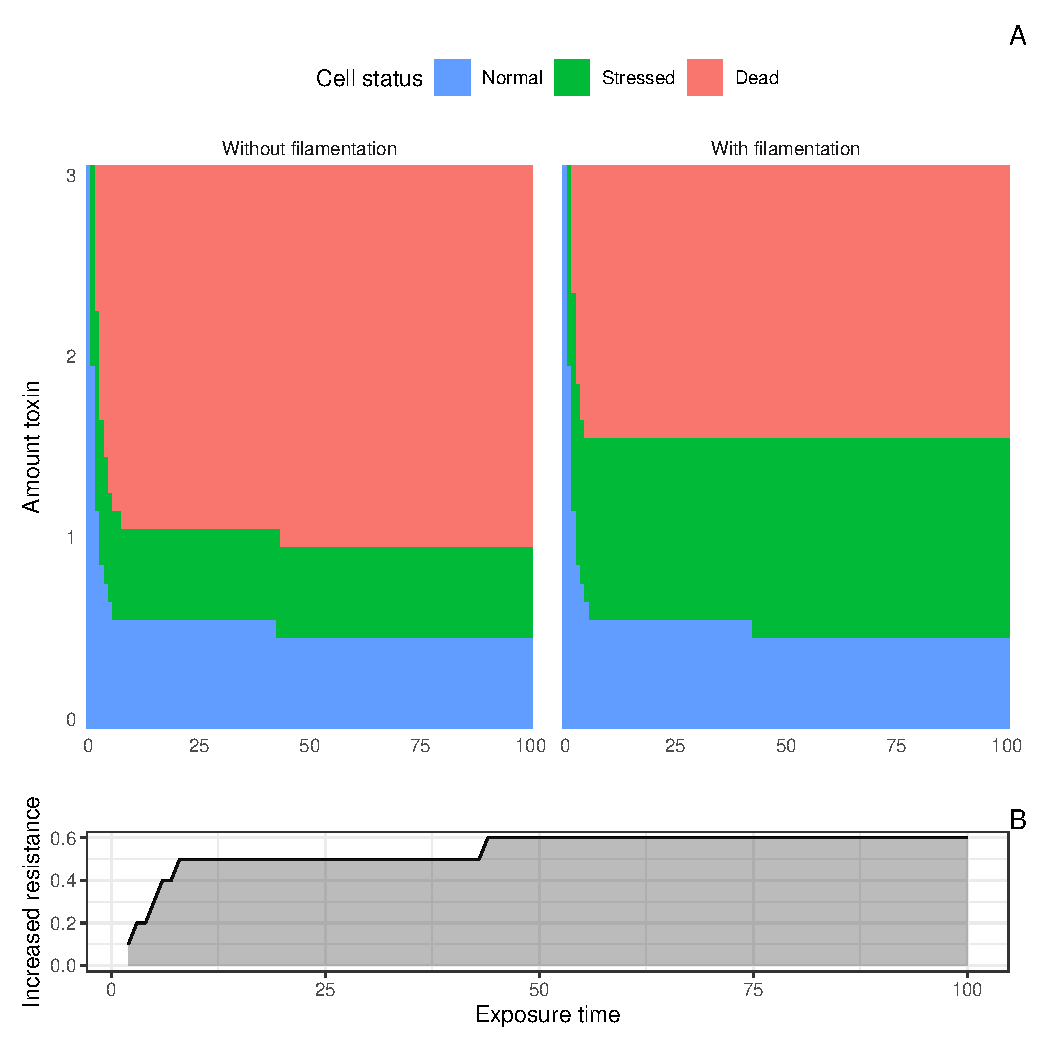
\includegraphics[width=1\linewidth]{downloadFigs4latex__main/increased-time-resistance} \caption[Effect of filamentation on minimum inhibitory concentration (MIC).]{\textbf{Effect of filamentation on minimum inhibitory concentration (MIC).} By exposing a cell to different toxin concentrations with stable signals, the cell achieves a set MIC for conditions without or with filamentation (separation between stressed and dead state) for each exposure time, without representing a change for the normal state cells' points (blue zone). Thus, the green line represents a gradual MIC increase when comparing each MIC between conditions for each exposure time.}\label{fig:increased-time-resistance}
\end{figure}

\hypertarget{heterogeneity-in-the-toxin-antitoxin-system-represents-a-double-edged-sword-in-survival-probability}{%
\subsection{Heterogeneity in the toxin-antitoxin system represents a double-edged sword in survival probability}\label{heterogeneity-in-the-toxin-antitoxin-system-represents-a-double-edged-sword-in-survival-probability}}

One of the SOS response system properties is that it presents synchronous activation times within homogeneous populations \autocite{friedmanPreciseTemporalModulation2005}. It has constant gene expression rates that help it cope with stress; however, it is possible to introduce variability by considering having multicopy resistance plasmids \autocite{million-weaverMechanismsPlasmidSegregation2014}. Therefore, the response times would have an asynchronous behavior at the global level but synchronous at the local level.

To include this observation into the model, we include a negative term to the internal toxin representing a toxin-antitoxin system. Therefore, the model now has an efficiency rate of the antitoxin and a stable amount per cell. We simulate the effect of the toxin-antitoxin system variation within a \(1000\) cell population; we initialize each one with similar initial conditions, except for the amount of internal antitoxin, defined as \(T_{anti} \sim N(\mu, \sigma)\). Considering that \(T_{anti}\) values \(< 0\) are equal to \(0\). For each experiment,\(\mu = 25\), while it was evaluated in the range \([0-20]\). For the generation of pseudo-random numbers and to ensure the results' reproducibility, the number \(42\) was considered seed.

As shown in Figure \ref{fig:variability-toxin-antitoxin}, when we compare heterogeneous populations in their toxin-antitoxin system, we can achieve different population dynamics, that is, changes in the final proportions of cell states; normal, stressed, and dead. This difference is because the cell sometimes has more or less antitoxin to handle the incoming stress situation.





\begin{figure}[H]
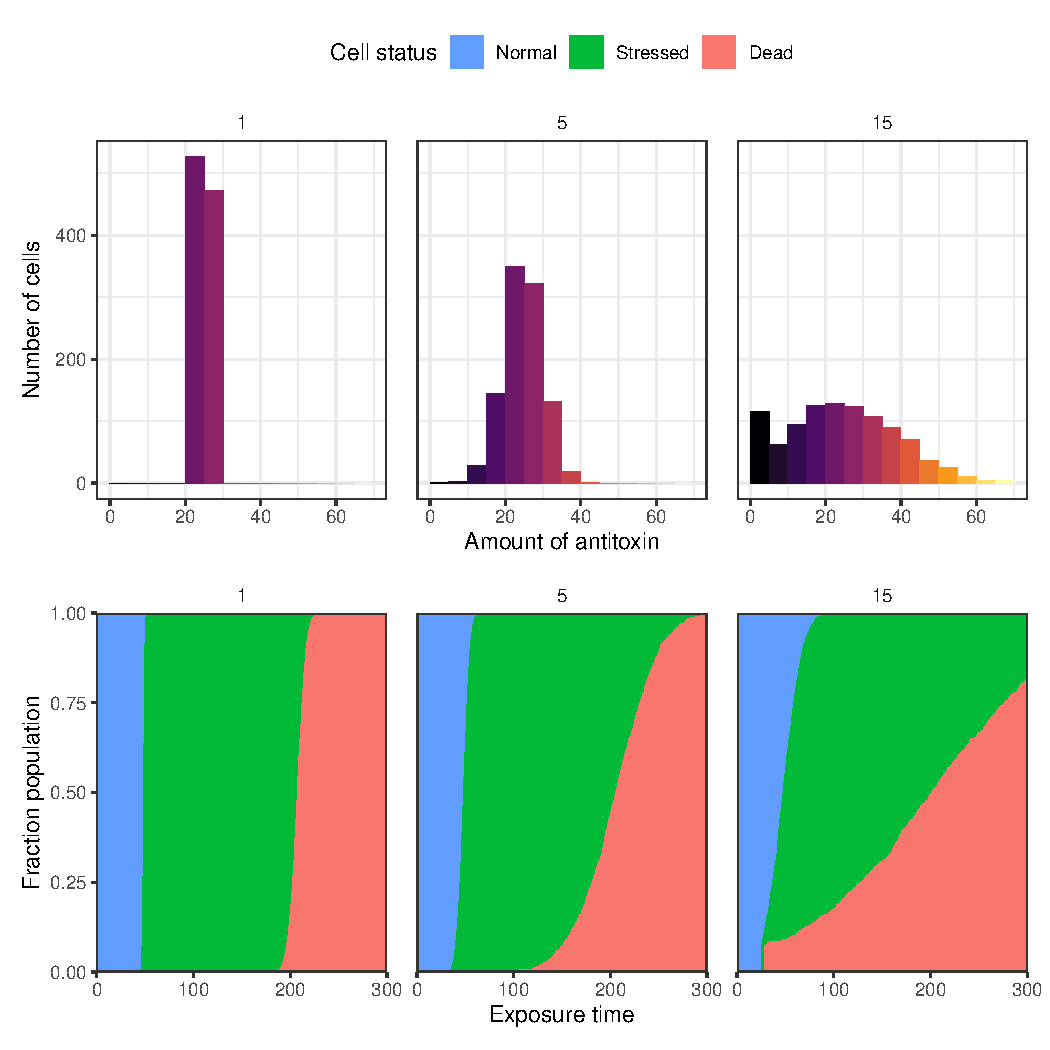
\includegraphics[width=1\linewidth]{downloadFigs4latex__main/variability-toxin-antitoxin} \caption[Variability in the toxin-antitoxin system produces different proportions of cell states.]{\textbf{Variability in the toxin-antitoxin system produces different proportions of cell states.} Histograms represent the distribution of antitoxin quantity, while the curves represent the population's fraction over time. The cell will start to filament after reaching a certain internal toxin threshold, \(T_{sos}\). Therefore, the expected global effect on the population's response times based on the amount of antitoxin is asynchronous, while at the local level, it is synchronous. Consequently, different proportions are presented in the cellular states since some cells will activate the filamentation system before and others later.}\label{fig:variability-toxin-antitoxin}
\end{figure}

Considering that the toxin-antitoxin system's variability can modify the proportions of final cell states, a question arose about heterogeneity levels' global behavior. To answer this question, we evaluate the probability of survival for each population, defined by its distribution of antitoxin levels. In this way, we characterized the population survival probability function into three essential points according to its effect: negative, invariant, and positive (see Figure \ref{fig:survival-probability}). Furthermore, these points are relative to the homogeneous population's death time in question (\(\tau_{kill}\)): when \(t < \tau_{kill}\) will represent a detrimental effect on survival, \(t = \tau_{kill}\) will be independent of variability, and \(t > \tau_{kill}\) will be a beneficial point for survival. Therefore, we concluded that the effect of heterogeneity in a toxin-antitoxin system represents a double-edged sword.





\begin{figure}[H]
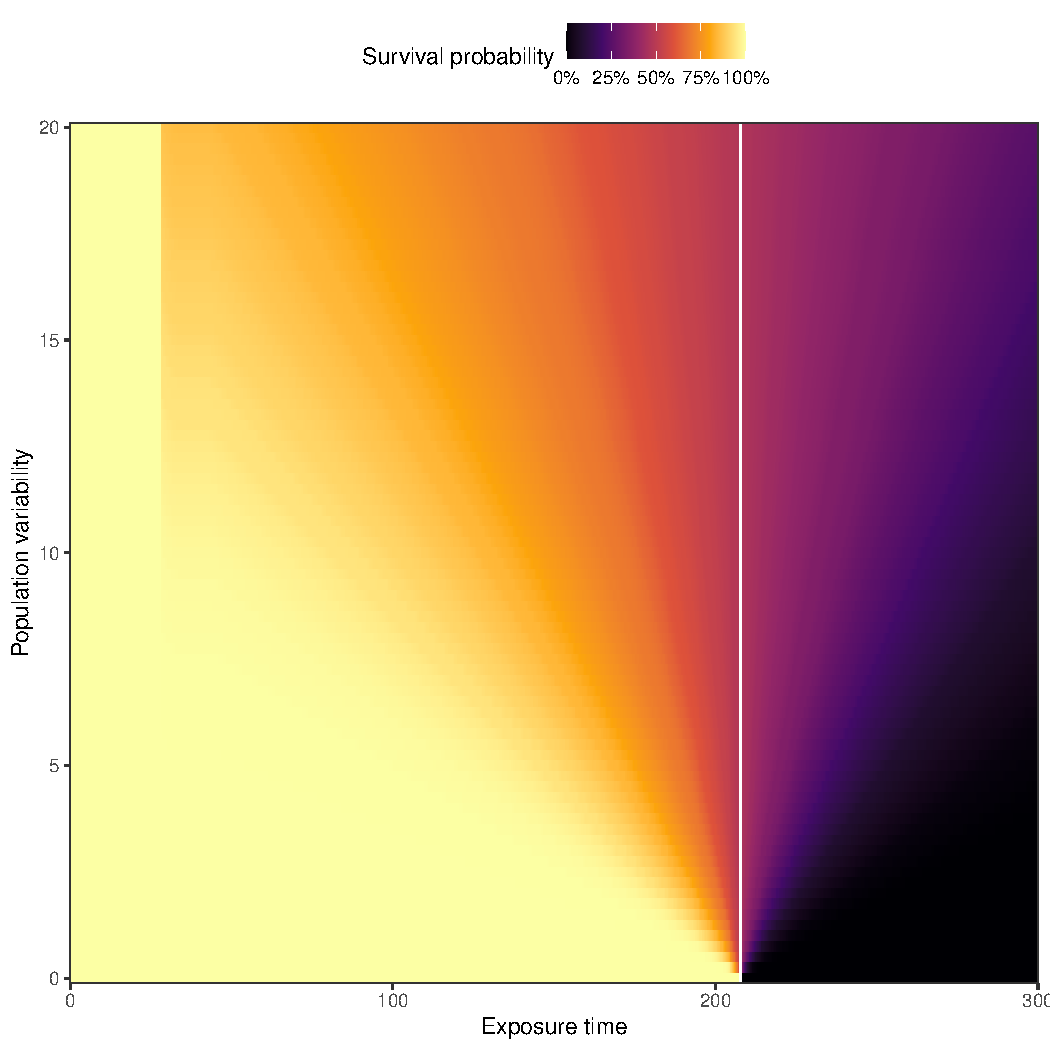
\includegraphics[width=1\linewidth]{downloadFigs4latex__main/survival-probability} \caption[Effect of variability on the toxin-antitoxin system.]{\textbf{Effect of variability on the toxin-antitoxin system.} The color of the heatmap is representative of the fraction of living cells at exposure time. The white vertical line represents the death time of the homogeneous population (\(\tau_{kill}\)). At \(t < \tau_{kill}\), it is shown that the fraction of survivors decreases as the variability in the population increases. When \(t = \tau_{kill}\), the variability does not affect the fraction of survivors, but it represents a percentage improvement for the homogeneous population. Finally, when \(t > \tau_{kill}\), the heterogeneity of the population favors survival.}\label{fig:survival-probability}
\end{figure}

\hypertarget{discussion-1}{%
\section{Discussion}\label{discussion-1}}

Today, there have been advancements in the number of techniques that have allowed it to extend quantitative analyses to individual cells' dynamic observations \autocite{camposConstantSizeExtension2014,meldrumFacultyOpinionsRecommendation2005,sliusarenkoHighthroughputSubpixelPrecision2011,taheri-araghiCellSizeControlHomeostasis2017,ursellRapidPreciseQuantification2017}. Therefore, studying their cellular behavior every day from medium to medium can be somewhat reproducible, facilitating the association of complex biological functions in simple mathematical equations \autocite{neidhardtBacterialGrowthConstant1999}.

Here, we proposed a mathematical model showing that filamentation could serve as a population's resilience mechanism to stress conditions. Finding that filamentation's net effect generates an additional window of time for the cell to survive, decreasing the toxin's intracellular concentration. However, we also found that a side effect of filamentation is to increase the cell's minimum inhibitory concentration. On the other hand, when we introduce variability in the amount of antitoxin in a cell population, we found that heterogeneity can be a double-edged sword, sometimes detrimental and sometimes beneficial, depending on the time of exposure to the toxic agent.

Due to the above, despite being simple, the model could have the ability to recapitulate the behavior seen in nature from variables that we can calculate easily with single-cell measurements. However, in other situations, it could be helpful to consider the addition of variables such as cell wall production and peptidoglycans' accumulation, among others. Notwithstanding the lack of parameters that are a little closer to reality, confirming that the model can work under experimental conditions would represent an achievement due to its explanatory simplicity, starting, in this way, the path of the study of filamentation oriented to the ecology of stress.

\hypertarget{chapter-discussion}{%
\chapter{Discussion}\label{chapter-discussion}}

\minitoc 

\noindent

\startappendices

\hypertarget{the-first-appendix}{%
\chapter{The First Appendix}\label{the-first-appendix}}


%%%%% REFERENCES
\setlength{\baselineskip}{0pt} % JEM: Single-space References

{\renewcommand*\MakeUppercase[1]{#1}%
\printbibliography[heading=bibintoc,title={\bibtitle}]}


\end{document}
